\documentclass[12pt]{article}
\usepackage{tikz}
\usepackage{pgfplots}
\usepackage{pgfplotstable}
\pgfplotsset{compat=1.13}

\usepackage{extsizes}
\usepackage{caption}
\usepackage{multirow}

\renewcommand{\epsilon}{\ensuremath{\varepsilon}}
\renewcommand{\phi}{\ensuremath{\varphi}}
\renewcommand{\kappa}{\ensuremath{\varkappa}}
\renewcommand{\le}{\ensuremath{\leqslant}}
\renewcommand{\leq}{\ensuremath{\leqslant}}
\renewcommand{\ge}{\ensuremath{\geqslant}}
\renewcommand{\geq}{\ensuremath{\geqslant}}
\renewcommand{\emptyset}{\varnothing}

\usepackage{geometry} % Простой способ задавать поля
\geometry{top=30mm}
\geometry{bottom=30mm}
\geometry{left=25mm}
\geometry{right=20mm}

\usepackage[T2A]{fontenc}			% кодировка
\usepackage[utf8]{inputenc}	
\usepackage[english,russian]{babel}   %% загружает пакет многоязыковой вёрстки
\usepackage{indentfirst}

\usepackage{amsmath,amsfonts,amssymb,amsthm,mathtools} 
\usepackage{graphicx}
\begin{document}
	\begin{minipage}{0.45\linewidth}
	Работу выполнил\\
	Самохин Валентин, 676 гр.\\[2mm]
	под руководством\\
	Артанова А.\,А\,.
	\end{minipage}
	\hfill
	\begin{minipage}{0.45\linewidth}\flushright
		Маршрут~IX \ №~8\\[3mm]
		12~апреля 2017~г.,\\
		\end{minipage}
		
		\vspace{8mm}
		\begin{center}
			\textbf{\Large Лабораторная работа №~2.2.1:}\\[\parskip]
			\LARGE Исследование взаимной диффузии газов
			\end{center}
			\vspace{0mm}
			
			\paragraph{Цель работы:}
			\begin{enumerate}
				\item регистрация зависимости концентрации гелия в воздухе от времени с помощью датчиков теплопроводности при разных начальных двалениях смеси газов;
				\item определение коэффициента диффузии по результатам измерений.
			\end{enumerate}
			
			\paragraph{В работе используются:}
			измерительная установка; форвакуумный насос; баллон с газом (гелий); манометр; источник питания; магазин сопротивлений .
			
			
			\vspace{2\parskip}
		\paragraph{Теоретическая справка.}
		В двухкомпонентной системе плотность потока вещества любого компонента в
		результате взаимной диффузии определяется законом Фика:
		\begin{equation}
		j_i = -D_{ij} \dfrac{\delta n_i}{\delta x},
		\end{equation}
		причём $D_{ij} = D_{ji} \equiv D$~--- коэффициент взаимной диффузии
		компонентов.
		
		Пусть два сосуда с объёмами $V_1, V_2$ соединены трубкой длины~$l$, сечения~$S$
		и заполнены смесью двух газов при одинаковом давлении (чтобы исключить
		макроскопические течения), но с разной концентрацией компонентов, причём один
		из компонентов преобладает.
		Вследствие взаимной диффузии концентрации каждого из компонентов со временем
		выравниваются, однако удобно рассматривать только концентрацию
		\emph{<<примеси>>.}
		
		Будем исходить из того, что описанный процесс происходит в основном благодаря
		диффузии в трубке, и считать процесс установления квазистационарным, тогда
		\begin{equation}
		J = -DS \frac{n_1 - n_2}{l},
		\end{equation}
		где $n_i$~--- концентрация примеси в $i$-ом сосуде. С учётом сохранения
		вещества запишем
		\begin{align}
		\dfrac{d(n_1 - n_2)}{dt} = -\frac{n_1 - n_2}{l} DS \left(\frac{1}{V_1} +
		\frac{1}{V_2}\right)
		&\Rightarrow
		\Delta n \equiv n_1 - n_2 = \Delta n_0 \exp\left(-\frac{t}{\tau}\right),
		\\		
		\tau \equiv \frac{V_1 V_2}{V_1 + V_2}& \frac{l}{SD}.
		\end{align}
		
		Для измерения концентраций будем применять датчики теплопроводности, считая
		линейными зависимость сопротивления от температуры и коэффициента
		теплопроводности от разности концентрации (раскладывая по Тейлору до первого члена, такой точности в нашем опыте достаточно).
		
		\paragraph{Экспериментальная установка}
		
		\begin{figure}[h]
				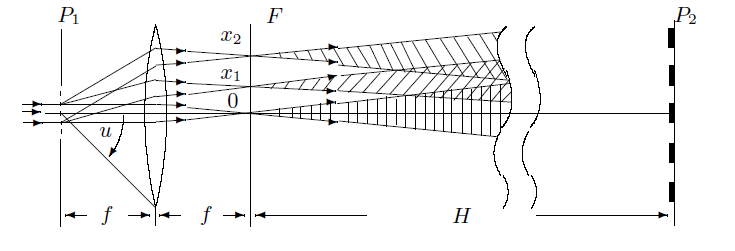
\includegraphics{1}
				\caption{Устройство установки}
		\end{figure}
\end{document}	